\documentclass[11pt]{extarticle}
\usepackage{fullpage}
\usepackage[ampersand]{easylist}
\ListProperties(Hide=10, 
Style*=$\bullet\;\,$, Style2*=$\;\,${\tiny$\blacksquare$}$\;\,$,Style3*=$\;\,${\large $\star$}$\;\,$,
Space*=0.5mm,Space2*=0mm, Space3*=0.5mm)

\usepackage{amsmath}
\usepackage{amssymb}
\usepackage{amsthm}
\newtheorem{thn}{Theorem}[]

\usepackage{mathtools}
\usepackage{bibref}

\usepackage{hyperref}
\hypersetup{colorlinks=true,
	linkcolor=black,
	filecolor=black,      
	urlcolor=black}
	
\usepackage{tikz}
\usetikzlibrary{calc}
\usetikzlibrary{shapes}
\usepackage{pgfplots}
\pgfplotsset{trig format plots=rad}

\usepackage[T1]{fontenc}
\usepackage[sc,osf]{mathpazo}
\usepackage{eulervm}

\usepackage{multicol}
%\setlength{\columnsep}{0.5cm}
\setlength\columnseprule{.1pt}

\newcommand{\ddsum}[3]{\displaystyle\sum_{#1=#2}^{#3}}
\newcommand{\snote}[1]{{\footnotesize(#1)}}
\newcommand{\ra}{\rightarrow}
\newcommand{\w}[1]{\text{#1}}
\author{\textbf{Yashas.N}}
\title{Complex Analysis}
\date{}
\begin{document}
	\maketitle
	\boldmath

\begin{multicols}{2}

\section{Power Series}
	
\begin{easylist}
	& $P(z)=a_0+a_1z+a_2z^2+a_3z^3\dots= \ddsum{n}{0}{\infty} a_n z^n.$
	& If $P(z)$ converges at $z=a$ then it converges absolutely  for all $|z|<|a|.$
	& If $P(z)$ diverges at $z=d$ then it diverges absolutely  for all $|z|>|d|.$
	& If two power series $A(z)=\ddsum{n}{0}{\infty} a_n z^n$ and $ B(z)=\ddsum{n}{0}{\infty} b_n z^n$ agree on an infinite sequence ($\neq 0$) converging to zero then they are same i.e. $a_i=b_i \; \forall i.$
	& In general for $P_b(z)=\ddsum{n}{0}{\infty}a_n(z-b)^n$ above holds as in displacement or translation of $b$ to $0$ i.e. $P_b(z)=P(w)\; for \; w=z-b.$
	& if radius of convergence of $P(z)=\ddsum{n}{0}{\infty} a_n z^n$ is $R$ then:
	&& $R=\lim\limits_{n\rightarrow\infty}\left|\frac{a_n}{a_{n+1}}\right|.$
	&& $R=\lim\limits_{n\rightarrow\infty}\left|\frac{1}{{|a_{n}|}^{1/n}}\right|.$
	&& $R=\lim\limits_{n\rightarrow\infty}\left|\frac{1}{\; limsup\;{|a_{n}|}^{1/n}}\right|.$
	& Radius of convergence of the power series of $f(z)$ at $k$ is equal to distance between $k$ and closest singularity of $f(z)$ to $k.$
\end{easylist}

\section{Transformations}
\subsection{$Z^n.$}
\begin{easylist}
	& $w=z^n=r^ne^{in\theta}.$
	& so from above each $z$ is magnified $|z|^n$ times and rotated $n\; arg(z)$ times in the plane i.e.
	
	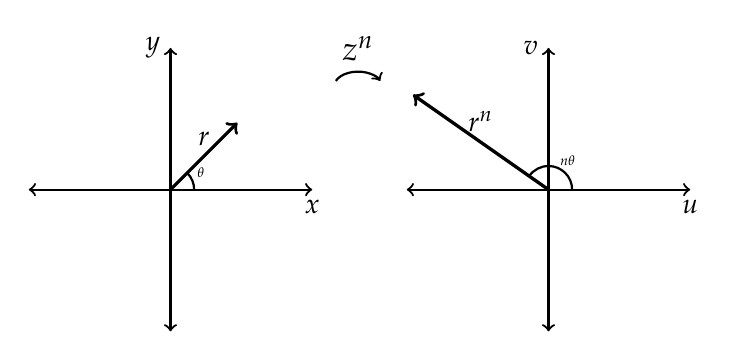
\begin{tikzpicture}[scale=0.6]
		\coordinate (a1) at (-4,0);
		\coordinate (wy) at (0,3);
		\coordinate (wx) at (3,0);
%		axes	
		\draw[thick,<->] ($(a1)+(wx)$) -- 
		node [below, pos=0]{$x$}
		($(a1)-(wx)$);
		\draw[thick,<->] ($(a1)+(wy)$) --
		node [left, pos=0]{$y$} 
		($(a1)-(wy)$);
%		z position
		\draw[very thick,->] (a1) -- 
		node [above,pos=0.5] {$r$}
		($(a1)+(45:2)$);
		
		\draw[thick] ($(a1)+(0.5,0)$) 
		arc [start angle=0, end angle = 45, radius=0.5]
		node [right] {\tiny$\theta$};
%		\node [above] at ($(a1)+(45:2)$) {$z$};

%		axes
		\coordinate (a2) at (4,0);
		\draw[thick,<->] ($(a2)+(wx)$) -- 
		node [below, pos=0]{$u$}
		($(a2)-(wx)$);
		\draw[thick,<->] ($(a2)+(wy)$) -- 
		node [left, pos=0]{$v$}
		($(a2)-(wy)$);
%		w position by z^n
		\draw[very thick,->] (a2) -- 
		node [above,pos=0.5] {$r^n$}
		($(a2)+(145:3.5)$);
		
		\draw[thick] ($(a2)+(0.5,0)$) 
		arc [start angle=0, end angle = 145, radius=0.5]
		node [above,pos=0.25] {\tiny$n\theta$};
		%		\node [above] at ($(a2)+(145:3)$) {$w$};
		
		\draw[thick,->] ($(a1)+(wx)+(0.5,2.3)$) 
		arc [start angle=160, end angle=20, x radius=0.5 , y radius =0.3]
		node [above, pos = 0.5] {\large$z^n$};
	\end{tikzpicture}
	 
& Images of circles are circle (with expanded or contracted radius),lines are lines
& Most geometric shapes just expand/diminished (amplified) and gets rotated (twist)

\end{easylist}
	
\subsection{$e^z.$}
\begin{easylist}
	& $w=e^z=e^xe^{iy}= e^x\cos{y}+i\;e^x \sin{y}=u+iv.$
	& $e^z=1+z+\frac{z^2}{2!}+\frac{z^3}{3!}+\dots \\$ and radius of convergence =$\infty.$
	& $e^z$ takes all values in $\mathbb{C}$ infinitely many times except zero i.e. range($e^z$)=$\mathbb{C}-\{0\}.$ 
	& if $x$ is constant then $u^2+v^2=e^x=r \\ \implies$ horizontal lines are mapped to circle.
	& if $y$ is constant then $\frac{v}{u}=\tan{y} $ or $ v=cu \\ \implies$ vertical lines are mapped to lines passing through origin (not including the origin).
	& every other line is mapped to a spiral centred at origin (not including). 
	 
	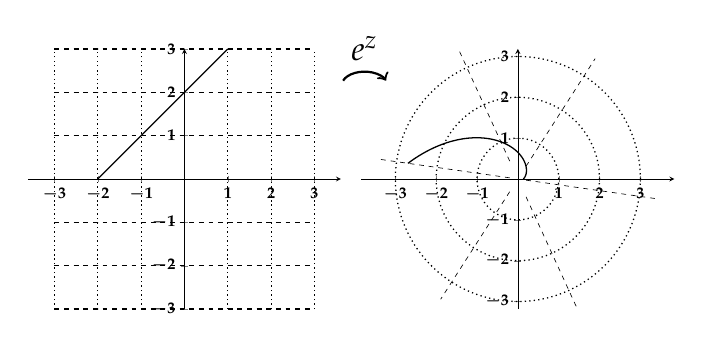
\begin{tikzpicture}[scale=0.58]
%		grid
		\begin{axis}[axis lines=middle, 
			axis equal,
			tick label style = {font=\boldmath},
			xtick ={-3,-2,-1,0,1,2,3},
			ytick ={-3,-2,-1,0,1,2,3},]
			\foreach \x in {1,2,3}{
				\addplot[dashed,thick,domain=-3:3,variable=t] ({t},{\x});
				\addplot[dashed,thick,domain=-3:3,variable=t] ({t},{-\x});
				\addplot[dotted,thick,domain=-3:3,variable=t] ({\x},{t});
				\addplot[dotted,thick,domain=-3:3,variable=t] ({-\x},{t});
			}
%			line
			\addplot[thick,domain=-2:1] {x+2};
		\end{axis}
		\draw[thick,->] (6.9,5) 
		arc [start angle=160, end angle=20, x radius=0.5 , y radius =0.3]
		node [above, pos = 0.5] {\large$e^z$};  
%		cicles
		\begin{axis}[axis lines=middle, 
			axis equal,
			tick label style = {font=\boldmath},
			xshift=7.3cm,
			xtick ={-3,-2,-1,0,1,2,3},
			ytick ={-3,-2,-1,0,1,2,3}]
			\foreach \a in {1,2,3}{
				\addplot[dotted,samples=50,smooth,thick,domain=0:2*pi,variable=t] ({\a*cos(t)},{\a*sin(t)});
				
				\addplot[ dashed,domain=0.2:3.5/(1+tan(\a)^2)^(1/2)] 
				{tan(\a)*x};
				\addplot[ dashed,domain=-0.2:-3.5/(1+tan(\a)^2)^(1/2)] 
				{tan(\a)*x};
			}
%			spiral
			\addplot[thick,smooth,samples=100,domain=-2:1,variable=s] ({e^s*cos(s+2)},{e^s*sin(s+2)});
	    	\end{axis}
    \end{tikzpicture}
     
\end{easylist}
\subsection{Trigonometric functions}
	\begin{align*}
	\cos{(z)}& =1-\frac{z^2}{2!}+\frac{z^4}{4!}-\frac{z^6}{6!}\dots\\ 
	 & =\frac{e^{iz}+e^{-iz}}{2}\\
		\sin{(z)}&= z-\frac{z^3}{3!}+\frac{z^5}{5!}-\frac{z^7}{7!}\dots\\ 
		&= \frac{e^{iz}-e^{-iz}}{2i}
	\end{align*}
	\begin{easylist}
	& $\cos(z-\pi/2)=\sin(z).$
	& $\cosh{(z)}=\cos{(iz)}.$
	& $ \sinh{(z)}=-i\sin{(iz)}  .$
	
	& so exploring only one of trigonometric functions namely $\cos z$ is sufficient
	& now	$\cos(x+iy)=\frac{e^{ix}e^{-y}+e^{-ix}e^{y}}{2}\\
	=\frac{e^y+e^{-y}}{2}\cos(x)-i\frac{e^y-e^{-y}}{2}\sin(x)\\
	= \cosh y \cos x -i \sinh y \sin x= u+iv.$
	& for $z=x+iy$ and $ w=cos(z)=u+iv $ if $y=y_0.$ is kept constant then\\
	$\frac{u^2}{\cosh^2 y_0}+\frac{v^2}{\sinh^2 y_0} =1.$
	& so every horizontal line is transformed to an ellipse with foci's $\pm 1.$ \\
	(as $a=\sinh y_0\; b= \cosh y_0 \implies c= b^2-a^2 = 1 \text{ (unit from origin) so foci's = } (1,0),(-1,0).$)
	& similarly $x=x_0.$ is kept constant then\\
	 $\frac{u^2}{\cos^2 x_0}-\frac{v^2}{\sin^2 x_0} =1.$
	& so every vertical line is transformed to hyperbola with foci's $\pm 1.$
\end{easylist}
	 
	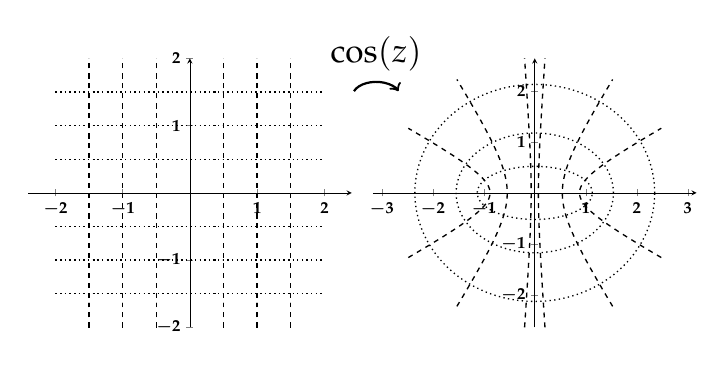
\begin{tikzpicture}[scale=0.6]
%	grid
		\begin{axis}[axis lines=middle, 
		axis equal,
		tick label style = {font=\boldmath},
		xtick ={-2,-1,0,1,2}]
		\foreach \x in {0.5,1,1.5}{
			\addplot[thick,dotted,samples=50,smooth,thick,domain=-2:2,variable=t] ({t},{\x});
			\addplot[thick,dotted,samples=50,smooth,thick,domain=-2:2,variable=t] ({t},{-\x});
			\addplot[dashed,samples=50,smooth,thick,domain=-2:2,variable=t] ({\x},{t});
			\addplot[dashed,samples=50,smooth,thick,domain=-2:2,variable=t] ({-\x},{t});
		}
		
	\end{axis}
	
	\draw[thick,->] (6.9,5) 
	arc [start angle=160, end angle=20, x radius=0.5 , y radius =0.3]
	node [above, pos = 0.5] {\large$\cos(z)$};  
%	ellipse, hyperola
	\begin{axis}[axis lines=middle, 
		axis equal,
		tick label style = {font=\boldmath},
		xshift=7.3cm]
		%		xtick ={-2,-1,0,1,2}]
		\foreach \x in {0.5,1,1.5}{
			\addplot[thick,dotted,samples=120,smooth,thick,domain=0:2*pi,variable=t] ({cosh(\x)*cos(t)},{sinh(\x)*sin(t)});
			
			\addplot[ dashed,samples=50,smooth,thick,domain=-1.7:1.7,variable=t] ({cos(\x)*cosh(t)},{sin(\x)*sinh(t)});
			
			\addplot[ dashed,samples=50,smooth,thick,domain=-1.7:1.7,variable=t] ({-cos(\x)*cosh(t)},{sin(\x)*sinh(t)});
		}
	\end{axis}
	\end{tikzpicture}
	 
	

\subsection{$\log(z).$}
\begin{easylist}
	& it denotes the inverse function of exponential
	& $\log(re^{i\theta})=ln(r)+i\theta.$
	& Clearly $\log$ is a multifunction as $\log(re^{i\theta})=ln(r)+i(\theta+2n\pi).$
	& properties of multifunctions:
	&& a region in range where multifunction takes ordinary single value is called a branch.
	&& typically branches are connected regions (simply or multiply)
	&& $q$ is branch point of multifunction if after a revolution around the point in domain the multifunction changes its values on the original observed point 
	&& $q$ is algebraic branch point of $f(z)$ if $f(z)$ returns to original observed value after $N$ revolutions around $q$, its order is $N-1$, a simple branch point has order 1.
	&& $q$ is logarithmic branch point if order is $\infty$ i.e. the original value is not restored by any number of revolution around the point.
	&& any curve drawn from branch point to $\infty$ is called a branch cut, typically is -ve real axis.
	&& eg: $z^{\frac{m}{n}}$ is one$-n$ mutifunction has branch point $0$ of order $n-1$, $z^\tau$ for $\tau$ irrational has logarithmic branch point of $0.$,
	&& a function can have more than one branch point eg: $\sqrt{z^2+1}=\sqrt{(z-i)(z+i)}$ has $\pm i$ as simple branch points.
	&& if a complex function or a branch of multifunction can be expressed as power series then the \textbf{radius of convergence} is distance to the nearest singularity or branch point.
	& $log(z)$ has logarithmic branch point at $0.$
	& $Log(z)=ln|z|+iArg(z)$ where the branch cut is -ve real axis and $-\pi < Arg(z)\leq \pi$ is called principle branch.
	& continuity of $Log(z)$ breaks down at $Arg(z)=\pi.$
	& $Log(1+z)=z-\frac{z^2}{2}+\frac{z^3}{3}-\frac{z^4}{4}+\dots$ is a power series centered at $1$ with radius of convergence $1$ converges on this unit circle except for $z=-1.$ 
	& other branches of $log(z)$ can be explored by writing $log(z)=Log(z)+2n\pi i.$
	& $z^k=e^{klog(z)}=e^{2n\pi k i} e^{kLog(z)}=e^{2n\pi k i}[z^b]$ where $[z^k]$ denotes root in principle branch. thus 
	&& $z^{p/q}=e^{p/q\;2n\pi i} [z^{p/q}].$
	&& Now for  complex powers
	\end{easylist}
	\vspace*{-1em}
	{\small
		\begin{align*}
		[z^{a+ib}]&=e^{(a+ib)(Log(z))}\\
		&=e^{(a+ib)(ln(r)+i\theta)}\\
		&= e^{a\;ln(r)}e^{-b\theta}e^{i(a\theta+b\;ln(r))}
		\end{align*}}
		\vspace*{-1em}
\[	\text{so }	[z^{a+ib}]=|z|^a e^{-b\;Arg(z)}e^{i(a\;Arg(z)+b\;ln|z|)}\]
	\[\text{ and }  z^{a+ib}=e^{i2\pi na}e^{-2\pi nb}[z^{a+ib}]\]
	
	
\subsection{Geometric transforms}
\begin{easylist}
	& translation by $v$ : $J_v(z)=z+v$ translates $0\rightarrow v.$
	& rotation about origin by $\theta $ : $R_0^\theta(z) =e^{i\theta}z.$
	& rotation about $w$ by $\theta .$ : \\
	$R_w^\theta=J_w \circ R_0^\theta \circ J_{-w}(z).$
	& Properties:
	&& $\{J_w\}$ forms a group under composition
	&& $R_w^\theta=J_v\circ R_0^\theta$ where $v= w(1-e^{\theta})\\.$
	i.e. rotation about any point is equal to a rotation around origin proceeded by translation.
	&& $R_a^\theta\circ R_b^\phi=R_c^{\theta+\phi}$ where $c=\frac{ae^{i\phi}(1-e^{i\theta})+b(1-e^{i\phi})}{(1-e^{i(\theta+\phi)})}.$
	&& if $\theta+\phi = 2n\pi$ then $R_a^\theta\circ R_b^\phi=J_v$ where $v=(b-a)(1-e^{i\phi}).$
	& Reflection about a line $L_1=\mathfrak{R}_{L1}.$
	& Reflection about real axis $\mathfrak{R}_{y=0}= \overline{z}.$
	& Reflection about line $ax+by=c$ is 
	\[\mathfrak{R}_{ax+by=c}=\frac{(b-ia) \overline{z}+2ic}{b+ia}.\]
	(can be done by transforming line to real axis by translation and rotation then conjugation and followed by inverse back to same line transformation).
	& Properties:
	&& If $L1$ and $L2$ intersect at $O$, and the angle from $L1$ to $L2$ is $\phi.$, then
	$\mathfrak{R}_{L2}\circ\mathfrak{R}_{L1}$ is a rotation of $2\phi$ about $O$ i.e. $R_{O}^{2\phi}.$
	&& If $L1$ and $L2$ are parallel, and $v$ is the perpendicular vector to both lines, connecting $L1$ to $L2$ (i.e. distance vector), then $\mathfrak{R}_{L2}\circ\mathfrak{R}_{L1}$  is a translation of $2v$ i.e. $J_{2v}.$
\end{easylist}
\subsection{$\frac{1}{z}.$}
\begin{easylist}
	& before studying $\frac{1}{z}$ we can study inversion about a circle :
	& $\mathfrak{J}_c(z)$ is the inversion of points in circle $c$ centered at $q$ with radius $R$ i.e. it transforms interior of circle to exterior and points on circle remain fixed 
	& some defining properties of $\mathfrak{J}_c$ (inversion of about circle $ c $ of radius $ R $ and centred at $ q .$) :
	&& $q\rightarrow\infty.$
	&& if $z$ is at distance $\rho$ from $q$ then it is moved to distance $R^2/\rho$ along same direction as $z$ from $q$ i.e.
	
	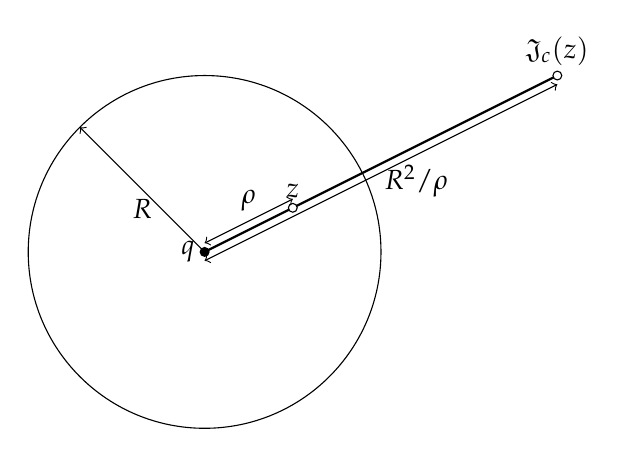
\begin{tikzpicture}[scale=0.56]
%		\draw[very thin,densely dashed] (-4,-4) grid (9,4);
		\draw (0,0) circle [radius = 4];
		\draw[fill=black]  (0,0) circle [radius=0.1];
		\node [left] at (0,0) {$q$};
		\draw[thin,->](0,0)--
		node [below, pos=0.5]{$R$}
		(-2.828,2.828);
		\draw [thick] (0,0)--(8,4);
		\draw[fill=white] (2,1) circle [radius=0.1]
		node [above] {$z$};
			\draw[fill=white] (8,4) circle [radius=0.1]
		node [above] {$\mathfrak{J}_c(z)$};
		\draw [thin,<->](0,0.2)--
		node [above,pos=0.5]{$\rho$}
		(2,1.2);
		\draw [thin,<->](0,-0.2)--
		node [below,pos=0.6]{$R^2/\rho$}
		(8,3.8);
	\end{tikzpicture}

	&& \[\mathfrak{J}_c(z)=\frac{R^2}{ \overline{z}- \overline{q}}\] (as $\overline{(z-q)}(\mathfrak{J}_c(z)-q)=R^2.$)
	& Properties of inversion \snote{$\mathfrak{J}_c$ centred $q$ radius $R.$}:
	&& inversion is involutory i.e. $\mathfrak{J}_c\circ\mathfrak{J}_c(z)=z$ or $\mathfrak{J}_c^2=I.$
	&& if $\tilde{a}=\mathfrak{J}_c(a)$ and $\tilde{b}=\mathfrak{J}_c(b)$ then $\bigtriangleup \tilde{a}q\tilde{b}$ is similar to $\bigtriangleup aqb.$
	&& every line that does not pass through $q$ is mapped to a circle passing through $q.$
	&&  as inversion is involutory it swaps the above point i.e. a circle passing through $q$ is mapped to a line not passing through $q.$
	&& A circle not passing through $q$ is mapped to another circle not passing through $q$ i.e. \textbf{inversion preserves circles}.
	&& if a circle $k$ cuts circle $c$ at $a$ and $b$ at right angles i.e. $k$ is orthogonal to $c$ then $k$ is mapped to itself i.e. \textbf{inversion maps orthogonal circles to $c$ to itself}.
	&& Inversion in a circle is anticonformal map
	&& If $a$ and $b$ are symmetric with respect to circle $k$ then their inversion images $\tilde{a}$ and $\tilde{b}$ are also symmetric with respect to the inversion image circle $\tilde{k}$ of $k.$
	&& i.e. Inversion maps any pair of orthogonal circles to another pair of orthogonal circles.
	&& also if $a$ and $b$ are symmetric w.r.t line $L_1$ (i.e. are reflections) then their inversion images are also symmetric to the inversion line $\tilde{L_1}.$ 
	& now $\frac{1}{z}=\overline{\left(\frac{1}{ \overline{z}}\right)}$ so $\frac{1}{z}$ is reflection of inversion centered at origin with unit radius on real axis, so all properties of inversion holds as reflection preserves shapes.
	&& now as both inversion and conjugation are anticonformal implies $1/z$ is a conformal map
	& define inverse point w.r.t. circle $C_{(z_0,R)}= \{z||z-z_0|=R\} $ as $ a $ and $ a^* $ are inverse points w.r.t $ C_{(z_0,R)} $ if $ a\mapsto a^* $ under $ \mathfrak{J}_{C_{(z_0,R)}}(z) $ i.e. if \\
	$ a^*=z_0+ \frac{ R^2 }{\overline{a-z_0}}$ or $ (a^*-z_0)\overline{(a-z_0)}=R^2. $ 
\end{easylist}	

\subsection{Mobius Transforms}
\begin{align*}
		M(z)&= \frac{az+b}{cz+d}\\
		&= \frac{a}{c}-\frac{ad-bc}{c^2}\left(\frac{1}{z+\frac{d}{c}}\right)\\
%		&\text{i.e.}\\
%		M(z)&=(\frac{a}{c}+z)\circ (-\frac{ad-bc}{c^2} z) \circ (\frac{1}{z}) \circ (z+\frac{d}{c})\\
		&= J_{a/c}\circ Az \circ \overline{\mathfrak{J}_u} \circ J_{d/c} (z)
\end{align*}
where $A=\frac{ad-bc}{-c^2}, u\equiv\{|z|=1\}.$
\begin{easylist}
& The only shape changing transformation in $M(z)$ is conjugate inversion, so all symmetries and properties of inversion follow to mobius transform.
& Properties
&& every mobius transform maps circles and straight lines onto circles and straight lines. 
&& above point may not be same order i.e. some circles can be mapped to straight lines and vis-a-viz. namely a
straight line or a circle maps onto a straight line if it passes through the point
$z =-d/c$, and onto a circle if it does not i.e. lines and circles not passing trough $ -d/c $ are mapped to circle.
&& mobius transform is conformal
&& more over mobius transforms are the only transforms that \textbf{map circles to circles}
&& To be specific A Mobius transformation maps an oriented circle $C$ to an oriented circle $\tilde{C}$ in such a way that the region to the left of $C$ is mapped to the region to the left of $\tilde{C}.$
&& Symmetric principle: If two points are symmetric with respect to a circle i.e. inverse points w.r.t a circle, then their images under a Mobius transformation are symmetric with respect to the image circle.
transformation are symmetric with respect to the image circle.
&& every mobius transform has only 2 fixed points
&& there exist a unique mobius transform sending any three points to any three points.
& the coefficients of a mobius transform $\{a,b,c,d\}$ are not unique as any $k\neq0.$
$\{ka,kb,kc,kd\}$ gives same mobius transform
& define cross ratio as $[z,a,b,c]=\frac{(z-a)(b-c)}{(z-c)(b-a)}.$
& $ p,q,r,s $ are mapped to $ \tilde{p},\tilde{q},\tilde{r},\tilde{s} $ by a Mobius Transformation iff 
\[[p,q,r,s]=[\tilde{p},\tilde{q},\tilde{r},\tilde{s}].\]
i.e. Mobius transforms are cross-ratio invariant.
& Unique Mobius transform $M(z)=w$ that transforms $a\rightarrow r,b\rightarrow s,c\rightarrow t$ is \[[w,r,s,t]=[z,a,b,c]\] or \[\frac{(z-a)(b-c)}{(z-c)(b-a)}=\frac{(w-r)(s-t)}{(w-t)(s-r)}.\]
\end{easylist}
\subsection{More on Mobius Transforms}
\begin{easylist}
	& now as coefficients of mobius transform are not unique if $ad-bc=1$ in $M(z)$ then we can associate a matrix for each of these mobius transforms from which resembling matrix properties can be associated to properties of transform i.e.
\end{easylist}
$M(z)=\frac{az+b}{cz+d} \leftarrow\!\rightarrow [M]
=\begin{bmatrix}
	a&b\\
	c&d\\
\end{bmatrix}.$
\begin{easylist}
	& Properties:
	&& $M_3=M_1 \circ M_2(z)$ them $[M_3]=[M_2][M_1].$
	&& if inverse of $M(z)$ is $M^{-1}(z)$ then $[M^{-1}]=[M]^{-1}.$
	&& identity transform $[I]=[1,0;0,1].$
	&& Thus $M(z)$ of form a group (for $ad-bc \neq 0,=1$) as $\mathbb{SL}(\mathbb{R},2)$ is a subgroup of $\mathbb{GL}(\mathbb{R},2).$ 
	& Homogeneous coordinates $z=\frac{\nu_1}{\nu_2}$ for $\nu_i\in \mathbb{C}.$
	& $[M]$ is a liner transform on homogeneous coordinates of $z$ that transforms homogeneous coordinates of  $ z $  to homogeneous coordinates of $M(z)$ i.e if $z=\nu_1/\nu_2$ , $M(z)=w=\rho_1/\rho_2.$ then
	\[
	\begin{bmatrix}
		a\quad&b\\
		c\quad&d\\
	\end{bmatrix}
	\begin{bmatrix}
		\nu_1\\
		\nu_2
	\end{bmatrix}
	=
	\begin{bmatrix}
		\rho_1\\
		\rho_2
	\end{bmatrix}.\]
	(although homogeneous coordinates may not be unique but their ratios ought to be )
	& Properties:
	&& $z=(\nu_1/\nu_2)$ is a fixed point of $M(z)$ iff $[\nu_1\quad\nu_2]^T$ is an eigenvector of $[M].$
\end{easylist}
\section{Automorphisms, Conformality and map of unit disks}
\begin{easylist}
	& any disk or half plain can be mapped to itself using mobius transform i.e. under specified mobius transforms say $ M_1 $ we can have $ M_1(D)=D $ for a disk $ D =\{z||z-a|\leq r\}$  and for $ M_2(\mathbb{H})=\mathbb{H} $ for any half plane $ \{z=x+iy| ax+by\geq c \} $ \snote{note : this is mere a bijection with restrictions, not the identity map in disk or half plane}.
	& more over the only conformal bijections (automorphisms) of disks $ \mapsto $ disks, 
	half planes $ \mapsto $ half planes are \textbf{Mobius Transforms only.} 
	& Let $C$ be a unit circle in $\mathbb{C}$ and $D$ be the unit disk it covers then :
	&& mobius transform's are the only automorphisms conformal on this unit disk
	&& this mobius automorphism's on unit disk has 3 degree of freedom (only 3 real numbers specify it)
	&& Now if two Mobius automorphisms on unit disk are say M and N map two interior points to same image points i.e. the agree on two interior points then M=N (as this takes 4 degree of freedom from both transforms)
	&& if $D$ is centered at origin then these 3 degrees of freedom are a point in $D$ ($a=(x+iy)$, $x,y \;\ra 2 $ degrees) that maps to origin and a point $e^{i\theta}$ on the disk $ C $ ($ \theta \; \ra 1$ degree) that $1$ is mapped to \snote{i.e. $ a=x+iy\mapsto 0,\; 1\mapsto e^{i\theta} $}.
	&& as $a$ is mapped to 0, and mobius transform preserves symmetry between points and their images (inversion) we have the point $1/ \overline{a}$ is mapped to $\infty$ (as $C$ maps to itself, $a,1/ \overline{a}$ are symmetric w.r.t $C$ their images should be  $0,\infty$).
	&& so now $a \mapsto 0\; \implies M(z)=\frac{k(z-a)}{d}$, $1/ \overline{a}\mapsto \infty\; \implies M(z)=k \frac{z-a}{ \overline{a}z-1}$ and as $M(1)\in C \; \implies |M(1)|=1\implies k=e^{i\phi}$ so the automorphism of unit disk \snote{|$z|\leq 1$} i.e. mobius transform is determined only by $a=x+iy \mapsto 0$ \snote{$ |a|<1 $} and $ p\mapsto 1 $ \snote{$ |p|=1 $} this is given by :
	\[ M_a^\phi(z)=e^{i\phi}\frac{z-a}{ \overline{a}z-1}.\]
	& now for \[ M(w)=\frac{ pz+q }{\overline{q}z+\overline{p}} \]for $ |p|>|q| $ then $ M(w) $ is an automorphism of unit disk \snote{transform this to $ M_a^\phi $ for $ a=q/p $ and $ e^{i\phi}=p/\overline{p} $. }
	& clearly $M_a^\phi(z)=e^{i\phi}M_a^0(z)$ so is just rotation of $M_a^0=M_a(z).$
	& properties of $M_a$ :
	&& $M_a$ is the only Mobius automorphism that swaps $a$ and $0$ (i.e. $M_a(a)=0,M_a(0)=a.$)
	&& now as an inversion about circle $ c $ maps circles orthogonal $ c $ to themselves (automorphism) thus automorphisms of unit circle can be viewed as inversions about circles orthogonal to unit circle to uncover this we break down that as $a\mapsto0$ and inversion circle is orthogonal to unit circle the center of inversion is on the line between $a$ to $0$ and as inversion is symmetric $1/ \overline{a}\mapsto \infty$ we conclude that center of inversion is $1/ \overline{a}.$
	&& as $M_a$ is conformal the above inversion should be coupled with reflection (on line perhaps) to give the exact map, as this reflection leaves $a,0$ fixed we conclude this is reflection about line $a$ to $0$ ($L_{a,0}.$)
	&& thus $M_a= \mathfrak{R}_{L_{a,0}}\circ \mathfrak{J}_{j}.$
	&& thus fixed points ($\pm \xi$) of $M_a$ is the intersection of $L_{a,0}$ and $j.$
	&& $M_a$ is Involutory.
	
	 
	\begin{flushleft}
			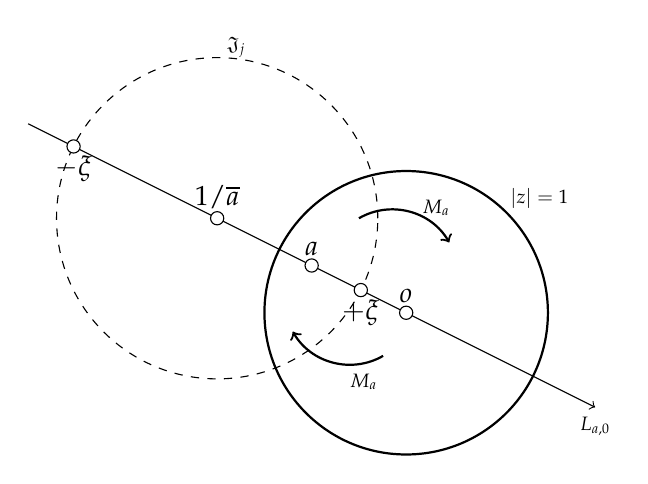
\begin{tikzpicture}[scale=1.2]
			%		\draw[dashed] (-4,3) grid (2,-2);
			\coordinate (q) at (-2,1);
			\coordinate (o) at (0,0);
			\coordinate (a) at (-1,0.5);
			\draw[dashed] (q) circle [radius=1.7];
			\node[above right] at (-2,2.6){\scriptsize$\mathfrak{J}_j$};
			\draw[thick] (o) circle [radius=1.5];
			\node[above right] at (1,1){\scriptsize$|z|=1$};
			\draw[->] (-4,2)--(2,-1)
			node [below,pos=1] {\scriptsize$L_{a,0}$};
			\draw[fill=white] (q) circle [radius =0.07]
			node[above] {$1/ \overline{a}$};
			\draw[fill=white] (o) circle [radius =0.07]
			node[above] {$o$};
			\draw[fill=white] (a) circle [radius =0.07]
			node[above] {$a$};
			\draw[fill=white] (-.48,.24) circle [radius =0.07]
			node[below] {$+\xi$};
			\draw[fill=white] (-3.52,1.76) circle [radius =0.07]
			node[below] {$-\xi$};
			\draw[thick,->] (-0.5,1) arc [start angle=120, end angle= 30, radius=0.7]
			node[above,pos=0.8]{\scriptsize$M_a$};
			\draw[thick,<-] (-1.2,-0.2) arc [start angle=210, end angle= 300, radius=0.7]
			node[below,pos=0.8]{\scriptsize$M_a$};	
		\end{tikzpicture}
	\end{flushleft}

	 
	& if $\mathbb{H}^\pm$ represents the upper or lower half plane ($Im(z) > 0 \; or\; < 0 $) , $\delta=\Delta(0,1)$ unit disk at origin  and $\partial\Delta =\{|z|=1\}$ then :
	&& for fixed $\beta \in \mathbb{C},\theta\in \mathbb{R}$ if $Im(\beta)>0$ then \[w=f(z)=e^{i\theta}\frac{z-\beta}{z-\overline{\beta}}.\]
	are the only conformal maps that maps \\
	$\mathbb{H}^+ \mapsto \delta$ , $\beta \mapsto 0$ and real line$ +\infty= \mathbb{R}_\infty \mapsto \partial \Delta$ (to see assume $|w|<1 \iff |z-\overline{\beta}|^2-|z-\beta|^2>0 \iff -2Re(z(\beta-\overline{\beta}))=4(Im(z))(Im(\beta))>0.$)
	& now if we use transform $R_0^\pi(z) = e^{i\pi}z=-z$ which rotates $\mathbb{H}^+$ to $\mathbb{H}^-$ we get $g=f\circ R_0^\pi (z).$ 
	\[ g(z)=e^{i\theta} \frac{z-b}{z- \overline{b}}.\]
	for $Im(b)<0$, are the only conformal maps that map 
	$\mathbb{H}^- \mapsto \delta$ , $b \mapsto 0$ and $\mathbb{R}_\infty \mapsto \partial \Delta.$
	& similarly if $h(z)=f\circ R_0^{\pi/2}$ \[h(z)=e^{i\theta} \frac{z-\gamma}{z+\overline{\gamma}} .\]
	for $Re(b)>0$, are the only conformally maps that map
		Right half plane $(Re(z)>0)\mapsto \delta$ , $\gamma \mapsto 0.$
	& a Mobius transform $ w=az+b/cz+d $ maps $\mathbb{H}^+\mapsto \mathbb{H}^+$ iff $a,b,c,d\in \mathbb{R}, ad-bc > 0$ (i.e. automorphisms of $\mathbb{H}^+.$) 
	& similar to above point a Mobius transform $ w=az+b/cz+d $ maps $\mathbb{H}^-\mapsto \mathbb{H}^-$ iff $a,b,c,d\in \mathbb{R}, ad-bc < 0$ (i.e. automorphisms of $\mathbb{H}^-.$) 
\end{easylist}

\section{Stereographic projection}

\begin{easylist}
	& To visually represent the whole complex plane and the point $\infty$ Riemann project the whole complex plane to a sphere : Riemann sphere ($\Sigma$) centered at origin a unit radius in 3 dimensions where the $xy$ plane is $\mathbb{C}.$
	& The point $N=(0,0,1)$ (north pole) maps to $\infty$ (in a pseudo sense) and every other point ($z$) is mapped to ($\hat{z}$)the point of intersection of the Riemann sphere and the line  through $N$ and the point.
	& Properties:
	&& Unit circle $C=|z|=1$ remains fixed
	&& interior of $C$ is mapped to Southern hemisphere particularly $0\mapsto (0,0,-1)=S.$(south pole) 
	&& exterior of $C$ is mapped to Northern hemisphere
	&& A line in $\mathbb{C}$ is mapped to circle passing through $N$ particularly the tangent of this circle at $N$ is parallel to the line (in 3 dimensions)
	&& It is \textbf{conformal map} in accordance to an observer \textbf{from inside of} $\Sigma$.
	&& Stereographic projection is can be broken down as inversion in the plane through $\{N,z\mapsto\hat{z}\}$ : if $K$ is a circle centered at $N$ of radius $\sqrt{2}$ in the plane where line through $N$ and $z$ passes then $\hat{z}$ is the image $\mathfrak{J}_K(z)$ in this plane (this plane is considered as $\mathbb{C}$ for $\mathfrak{J}_K(z).$)
	&& From above it is clear that Circles are mapped to circles in particular origin centered circles are mapped to horizontal circles (i.e circles in planes parallel to $xy.$ plane)
	& Properties related to functions:
	&& Complex conjugation in $\mathbb{C}.$ induces a reflection of the Riemann sphere in the vertical plane passing through the real axis.
	&& Inversion of $\mathbb{C}$ in the unit circle induces a reflection of the Riemann sphere in its equatorial plane (i.e. Northern hemisphere $\leftarrow\!\rightarrow$ Southern Hemisphere).
	&& The mapping $z \rightarrow (1/z)$ in $\mathbb{C}$ induces a rotation of the Riemann sphere about the real axis through an angle of $\pi.$
	&& properties functions like conformality at $\infty$ can be checked through Stereographic projection.
	& formulas of Projection
	&& if $z \mapsto (X,Y,Z)$ then:
	&& { \Large$Z=\frac{|z|^2-1}{|z|^2+1}$ , $X+iY=\frac{2z}{1+|z|^2}=\frac{2x+i2y}{1+x^2+y^2}.$}
	&& if  $z \mapsto (\theta,\phi)$  for $\theta $ angle subtended around $z$ axis in $xy$ plane and $\phi$ angle subtended at center by $N$ and $\hat{z}$ then:
	&& {\Large$z=\cot(\phi/2) e^{i\theta}$} or\\ $\theta= Arg(z),\quad\phi = 2\cot^{-1}(|z|).$
\end{easylist}
\section{Analyticity}
\begin{easylist}
	& if $z(x+iy)\mapsto f(z)=w(u+iv)$ then $df=du+idv$ $du=\frac{\partial u}{\partial x}dx+\frac{\partial u}{\partial y}dy$ and  $dv=\frac{\partial v}{\partial x}dx+\frac{\partial v}{\partial y}dy$ i.e.
\end{easylist}
	\[
	\begin{bmatrix}
		du\\
		dv
	\end{bmatrix}
	=
	\begin{bmatrix}
		\partial_x u & \partial_y u\\
		\partial_x v & \partial_y v
	\end{bmatrix}
	\begin{bmatrix}
		dx\\
		dy
	\end{bmatrix}.
	\]
\begin{easylist}
	& where the linear transform is the Jacobian matrix of $f.$
	& now in $\mathbb{C}$ if $df(w)=f'(z)dz$ to be true $f'(z)$ should not depend on $dz$ i.e. each infinitesimal vector $dz$ at $z$ should transform to $dw$ at $w=f(z)$ by the same factor $f'(z)$ no matter the direction of $dz.$.
	& this condition tells us that $dw$ is just the amplification and rotation or twist or together \textbf{amplitwist} of $dz$ (as $f'(z)\in \mathbb{C}\; \implies dw=f'(z)dz=r'e^{i\theta'}dz.$) 
	& now if $f$ is diffrentiable at $z$ then $f'(z)$ exist so the infinitesimal map at point $z$ is an amplitwist.
	& clearly amplitwist is conformal (as amplification and twist is)
	& now for the converse if a map is conformal at $z$ then it is not presupposed to be amplitwist at $z$ as the amplification may vary but if we presuppose that the map is locally conformal at $z$ (i.e in some whole neighborhood) then clearly the map is locally amplitwist at $z$ (as infinitesimal $\bigtriangleup$ is mapped to similar infinitesimal $\bigtriangleup$).
	& By above we define \textbf{Analytic functions} : functions in $\mathbb{C}$ whose effect are locally (infinitesimal) an amplitwist or a function is analytic at $z$ if it is diffrentiable at $z$ and in a neighborhood of $z.$ (as diffrentiable in neighborhood makes it locally conformal).
	& Thus we have an \textbf{Analytic function is Conformal}.
	& Geometric properties of Analytic function:
	&& infinitesimal circles are mapped to infinitesimal circles 
	&& A mapping between spheres represents an analytic function iff
	it is conformal.
	&& Conformality of analytic functions breakdown near critical points ($f'(z)=0.$) and branch points.
	& Geometric property of general transform on $\mathbb{C}$: as jacobian is a linear transform by singular value decomposition of $2\times2$ matrices we have the local linear transform by a complex mapping is a stretch in direction $(d)$, another stretch in direction perpendicular to in $(d^\perp).$ and finally a twist. in particular an infinitesimal circle is transformed to an ellipse (may not be conformal).
	& \textbf{C-R equations} :
	&& now as $f$ is analytic $\implies f'(z) \in \mathbb{C}$ so multiplying by Jacobian matrix is equivalent to a complex multiplication now as 
\end{easylist}
	$(a+ib)(x+iy)=(ax-by)+i(bx+ay)\\
	 \leftarrow\!\rightarrow 
	\begin{bmatrix}
		a & -b\\
		b & a
	\end{bmatrix}
	\begin{bmatrix}
		x\\
		y
	\end{bmatrix}
	= 
	\begin{bmatrix}
		ax-by\\
		bx+ay
	\end{bmatrix}\\.$ 
we have 
$J=	\begin{bmatrix}
	\partial_x u & \partial_y u\\
	\partial_x v & \partial_y v
\end{bmatrix}=
\begin{bmatrix}
		a & -b\\
		b & a
\end{bmatrix}.$
i.e. 
\[\partial_x u = \partial_y v \, , \quad \partial_y u = - \partial_x v.\]
\[i\partial_x f = \partial_y f.\]
which gives the Cartesian-Cartesian form(C-C)
now in Polar-Cartesian (P-C) form we have $f(re^{i\theta})=u+iv$ and C-R equations are 
\[\partial_\theta v = r \partial_r u\, , \quad \partial_\theta u=-r\partial_r v.\]
\[ \partial_\theta f=ir\partial_r f.\]
(P-P) form  $f(re^{i\theta})=Re^{i\Psi}$ C-R equations
\[\partial_\theta R=-rR \partial_r\Psi\, , \quad R\partial_\theta \Psi=r\partial_r R.\] 
(C-P) form  $f(x+iy)=Re^{i\Psi}.$ C-R equations
\[\partial_x R=R\partial_y \Psi \, ,\quad \partial_y R=-R \partial_x \Psi.\]

\begin{easylist}
	& General properties of Analytic functions:
	&& if $f,g$ are analytic then $f+g,f\times g,f\circ g,f^{-1}$ are analytic when ever they are defined,  in particular as $f$ is amplitwist locally there is a 1-1 correspondence in a neighbourhood of non critical points to their images $\implies$ that local inverse exists. 
	&& if $f$ is analytic in $E$ then so is $f'$ (i.e. $f$ is infinitely differentiable in the defined region)
	&& every zero or an analytic point is isolated (generally $p$-point of $f$ or pre-image of $p$ in $f$ doesn't have a limit point.)
	&& \textbf{Identity/Uniqueness Theorem}: restating the above we have, if $f(z)$ is analytic in $D$ and if $S$ set of zeroes of $ f(z) $ and if $ S $ has a limit point in $D$ then $f(0)\equiv 0$ in $D$ (in general if $p$-points of $f$ has a limit point then $f(z)\equiv p$).
	&& Extending the above we get, if even an arbitrarily small segment of curve is crushed to a point by an analytic mapping, then its entire domain will be collapsed down to that
	point (i.e. the function is constant) (this property is known as \textbf{Rigidity})
	&& from above if $f,g$ analytic agree on a curve or more generally $\{a_n\}\mapsto a$ then $f\equiv g.$ 
	&& if some identity of analytic function $f(z)$ holds when restricted to $\mathbb{R}$ then it holds for entire $\mathbb{C}.$ (eg: odd and evenness.)
	
\end{easylist}

\section{Analytic continuation}
\begin{easylist}
	& an analytic function or a power series can be extended (from defined) to other regions this is analytical so called Analytic continuation.
	& Analytic continuation via reflection:
	&& if $f$ is an generalization of a real function (defined on $\mathbb{R}$) and is known in upper or lower parts of real axis (in some region with some parts of $\mathbb{R}$ as boundary) then it can be \textbf{analytically continued by} $f*(z)=\overline{f( \overline{z})}$ in the other half part (reflection by $ \overline{z}$  part of region)(this holds by property of rigidity of analytic functions).
	&& In general if $f$ maps a line ($L$) to another line ($\hat{L}$) then we can analytically continue one side of $L$ to the other by using the fact that points symmetric in $L$ map to points symmetric in $\hat{L}$.
	&& similarly if $f$ maps a circle $C$ to circle $\hat{C}$ then mobius transforms can be used to translated these to symmetries i.e. $M:C\mapsto L$, $\hat{M}:\hat{C}\mapsto\hat{L}$ (as composition by mobius transfor ehic are analytic doesnt change the analyticity of $f \mapsto \hat{M}\circ f \circ M^{-1}$).
	& \textbf{Schwarzian Reflection}:
	&& Given a sufficiently smooth curve $K$, it is possible to find an analytic function $S_K(z)$ such that $z\in K\; \implies \; S_K(z)= \overline{z}$ then 
	&& Schwarz function of $K$ = $\tilde{z}=\Re_K(z)=\overline{S_K(z)}.$
	&& clearly if $q\in K\quad \tilde{q}=\overline{S_K(q)}=\overline{ \overline{q}}=q$ i.e. remains unchanged.
	&& Also as $S_K$ just amplitwists infinitesimal disk at $q\in K$ to infinitesimal disk in $ \overline{q}\in  \overline{K}$ we observe that for $S_K|qp\mapsto  \overline{q} \overline{p}$(for $p,q\in K , qp $ infinitesimal ) amplification $=1$ and twist $=-2\phi$  where $\phi$ is the angle b/w tangent to $K$ at $q$ with horizontal
	&& so from above we get if $ a $ is on infinitesimal circle passing through 
	$K$ then $\tilde{a}=\Re_K(a)$ is reflection along the tangent of $K$. i.e $\Re_K$ near $K$ is sort of like Reflection in $K$ (pseudo).
	&& $\Re_K$ is anticonformal so $\Re_K\circ\Re_K$ is conformal so analytic (as amplification=1) and as $\Re_K\circ\Re_K$ maps infinitesimal areas around $K$ to itself thus agrees with Identity so is Identity i.e. $\Re_K\circ\Re_K(z)=z$.
	&&  Now if $K$ is a smooth enough curve to posses $S_K$ and any analytical map $f$ defined on a region bordering $K$ such that $\hat{K}=f(K)$ also posses $S_{\hat{K}}$ then we can analytically continue $f$ around $K$ (reflection of region by $K$) by demanding points symmetric to $K$ are mapped to points symmetric to $\hat{K}$ by $f$ and this analytic continuation is given by:
	\[F=\Re_{\hat{K}}\circ f \circ \Re_K.\]
\end{easylist}

\section{Complex Integration}
\begin{easylist}
	& we define complex integration as the generalized Riemann Integration over a given path $a$ to $b$ or as contour integration
	& clearly integration here depends on path 
	& complex integration can be visualized as weighted vector sum :
	if $S$ is path from $a$ to $b$ and $\Delta_j$ 's are vector decomposition (partition of $S$ and linearly) that form $S$ , $w_j=f(mid\;\Delta_j)$ i.e $f$(mid points of $\Delta_j.$) then we can generalize as 
	\[\int_{S}f(z)dz=\sum_{j\rightarrow\infty}w_j\Delta_j\]
	& from above we get: if $|f|\leq M$ in image of $K.$ then
	\[\left|\int_{S}f(z)dz\right|\leq M . \text{length of }K.\]
	& \textbf{Winding number and properties }:
	& winding number for a closed loop $L$ and a point $a$ = $\nu(L,a)$ is the number of revolutions $z-a$ makes as it traces $L$ (where  we fixing a direction for counter-clockwise revolution is +ve and clockwise is -ve by convention)
	& A simple loop is a closed curve that doesnt intersect with itself
	& now as a point moves from left to right if it crosses a boundary of the loop and the loops direction is downwards (upwards) the winding number increased (decreases) by 1
	(here the first entry of the point to loop is made to be in loop moving in downwards direction).
	& we define inside of a loop $L$ to be regions (points) where $\nu[L,a]\neq 0.$
	& Hopf's degree Theorem(ristricted to $\mathbb{C}$): A loop $K$ may be continuously deformed into another loop $L$, without ever crossing the point $p$, if and only if K and L have the same winding number round p.
	& $d$ is a $p$-point of a function $f$ if set of pre-images of $p$ in $f$ contains $d$ i.e. $d \in {f^{-1}(p)}.$(pre-image)
	& \textbf{Argument-Principle} theorem: If $f(z)$ is analytic inside and on a simple loop $\Gamma$ , and $N$ is the number of $p$-points (counted with their multiplicities) inside $\Gamma$ , then $N = \nu(f(\Gamma), p]$.
	& if $f$ analytic, $f(a)-p=0$ and for $\Delta=z-a\quad f(a+\Delta)=p+\Omega(Z)\Delta^n$ (obtained by Taylor series) here algebraic multiplicity of $a$ in $f$ is $n$,
	for sufficiently small circle $C_a$ around $a$ that doesnt have any other $p$-points then
	 \begin{center}
		$\nu(f(C_a),a)=n.$
	\end{center} 
	i.e. $f(C_a)$ loops around $p$ exactly $n$ times.
	& now we define $\nu(a)$ for a continuous function $h$ as : if $h(a)=p$, $\Gamma_a$ is the loop having only $a$ and no other $p$-points then topological multiplicity $\nu(a)=\nu(h(\Gamma_a),a).$
	& clearly as analytical maps are conformal we have $\nu(a)$ is always +ve ($\neq 0.$ ) for analytic functions
	& $\nu(a)=\text{sign of }det(J(a))$ where $J$ is Jacobian 
	& \textbf{Topological Argument-Principle} theorem: for a continuous map $h$ the total number of $p$-points inside $\Gamma.$ (counted with their topological
	multiplicities) is equal to the winding number of $ h(\Gamma)$ round $p.$.
	& \textbf{Darboux’s Theorem }: If an analytic function h maps $\Gamma$ onto $ h(\Gamma)$ in one-to-one fashion, then it also maps the interior of $\Gamma$ onto the interior of 
	$ h(\Gamma)$ in one-to-one fashion.
	& \textbf{Rouche’s Theorem }: for $f,g$ analytic in and on $\Gamma$, If $|g(z)| < |f(z)|$ on $\Gamma$ , then $(f+g)$ must have the same number of zeros inside $\Gamma$ as $f$. 
	& \textbf{Brouwer’s Fixed Point Theorem} : any continuous mapping of the disc to itself will have a fixed point.\\
	In general there must be a fixed point if the disc is mapped into its interior and there are at most a finite number of fixed points. (now if the map is analytic then the number of fixed points inside the disk is only one).
	& \textbf{If f is analytic inside and on a simple loop $\Gamma$ then no point outside $f(\Gamma)$
	can have a pre-image inside $\Gamma$.}(i.e interior of $\Gamma$ maps to interior of $f(\Gamma).$)
	& \textbf{ Maximum Modulus Theorem} : The maximum (minimum respectively if $ f(z)\neq 0 $ inside the closed boundary) of $|f(z)|$ on a region where $f$ is analytic is always achieved by points on the boundary, never ones inside.
	& \textbf{Schwarz's Lemma} : If an analytic mapping of the disc to itself leaves the center fixed,then either every interior point moves nearer to the center, or else the transformation is a simple rotation. (i.e. them map is contractive  towards the center).
	& \textbf{General Schwarz's Lemma} : \\
	If $f:\Delta(\{|z|<1\}) \mapsto \overline{\Delta}$ is analytic and has a zero of order $n$ at origin then:
	&& \[|f(z)|\leq |z|^n \; \forall z\in\Delta.\]
	&& \[|f^n(0)|\leq n!\]
	&& if Equality holds (any one) for any point inside $\Delta$ other than $0$ then $f(z)=az^n,|a|=1.$
	& modifying Schwarz's lemma we get for $ f $ analytic in $ \Delta(a,R) $ , $ |f(z)|\leq M $ in $ \Delta(a,R) $ and $ f(a)=0 $ then (applying Schwarz's lemma for $ g(z)=f(Rz+a)/M $ i.e. $ z\ra Rz+a $ for $ |z|<1 $)
	&& \[|f(z)|\leq \frac{  M|z-a|  }{R} \] for every $ z\in \Delta(a,R) $.
	&& \[|f'(a)|\leq \frac{ M }{R} .\]
	&& and if equality holds for any two then $ f=M\epsilon(z-a)/R $ for some $ |\epsilon|=1 .$ 
	& \textbf{Schwarz-Pick Lemma} : Unless an analytic mapping of the unit disc to itself is a automorphism the hyperbolic separation of every pair of interior points decreases.
	\\ i.e.\\ 
	if $f$ is analytic on $\Delta$ , $|f(z)|\leq1 \forall z\in \Delta$ and $f(a)=b \text{ for some }a,b \in \Delta$, then
	\[|f'(a)|\leq \frac{1-|f(a)|^2}{1-|a|^2}.\]
	and for $a,a'\in \Delta$
	\[\rho(f(a),f(a'))\leq\rho(a,a').\]
	where $\rho(z,a)=|(z-a)/( \overline{a}z-1)|.$
	& \textbf{Liouville's Theorem} :An analytic mapping cannot compress the entire plane into a region
	lying inside a disc of finite radius without crushing it all the way down
	to a point, i.e. a bounded entire function is constant or bounded harmonic function is constant (by Taylor series)
	& \textbf{Generalized Liouville's Theorem } : if $f$ is an entire function such that $|f(z)|\leq M |z|^\alpha$ for all sufficiently large $|z|$ and $\alpha\geq 0,\; M>0$ then $f$ reduces to a polynomial of maximum degree $n$ closest integer to $\alpha$.
	& \textbf{Generalized Argument-principle theorem} :Let $f$ be analytic on a simple loop $\Gamma$ and analytic inside except for a finite
	number of poles. If $N$ and $M$ are the number of interior p-points and
	poles, both counted with their multiplicities, then $\nu(f(\Gamma ),p)= N-M.$
	& for any closed loop $L$ 
	$\oint_L \frac{1}{z} dz  = 2\pi i \nu(L,0)$
	in general 
	\[\oint_L \frac{1}{z-p} dz  = 2\pi i \nu(L,p).\]
	& now as $Im(a \overline{b})\equiv a\times b$ it gives $ 2\times$ the area enclosed by triangle formed by sides $a$ and $b$ vectors so we have for a simple loop $L$:
	\[ \oint_L  \overline{z}dz =2i\times \text{area enclosed by }L.\]
	for general loop $L$
	\[\oint_L  \overline{z}dz =2i\times\sum_{\text{inside}}\nu_j A_j.\]
	where $A_j$ is the area enclosed by points which have $\nu_j=\nu(L,p)=a \neq 0$  constant (i.e form a part of loop).
	
	& \textbf{Cauchy's Theorem} :If an analytic mapping has no singularities “inside” a loop, its integral round the loop vanishes (i.e. = 0).
	& from above we get in integral of analytic functions are \textbf{path independent}.
	& \textbf{Morera’s Theorem} :  If all the loop integrals of $f$ are known to vanish  in a region then $f$ is analytic in that region.
	& if $m\neq -1$ then
	\[\int\limits_{A}^{B}z^m dz= \frac{1}{m+1}(B^{m+1}-A^{m+1})\]
	& clearly from above we have \[\oint z^m dz=0 \text{ if m }\neq -1.\]
	& \textbf{Deformation Theorem }: If a contour sweeps only through analytic
	points as it is deformed, the value of the integral does not change.
	& \textbf{Cauchy's formula } : if $f(z)$ is analytic inside a simple loop $L$ then \[ f^n(a)=\frac{n!}{2\pi i}\oint_L\frac{f(z)}{(z-a)^{n+1}} dz.\]
	& \textbf{General Cauchy's theorem} : if $L$ is not simple then
	\[ \nu(L,a)f^n(a)=\frac{n!}{2\pi i}\oint_L\frac{f(z)}{(z-a)^{n+1}} dz.\]
	& \textbf{Taylor Series }: If $f(z)$ is analytic, and a is neither a singularity nor a branch point, then $f(z)$ may be expressed as the following power series, which converges to $f(z)$ within the disc whose radius is the distance from $a$ to the nearest singularity or branch point:
 \[ f(z)=\sum_{n=0}^{\infty} c_n(z-a)^n.\text{ where } \]
 \[c_n=\frac{f^n(a)}{n!}=\frac{1}{2\pi i}\oint_L \frac{f(z)}{(z-a)^{n+1}}dz.\]
 & \textbf{Laurent Series }: if $f$ is analytic inside an annulus centered at $a$ then $f$ an be expressed as the following series (for any simple loop $K$ inside the annulus)
 \[ f(z)=\sum_{-\infty}^{\infty} a_n(z-a)^n.\text{ where } \]
 \[a_n=\frac{1}{2\pi i}\oint_L \frac{f(z)}{(z-a)^{n+1}}dz.\]
 & \textbf{General Residue Theorem} : from Laurent series and integral of $z^m$ we have if $f$ is analytic then for a loop $L$ containing only isolated singularities $\{a_k\}$ of $f$, we have:
 \[\oint_L f(z)dz=2\pi i\sum_{k} \nu[L,a_k]Res(f,a_k).\]
 where $Res(f,a_i)=a_{-1}$ or coefficient of $1/(z-a_i)$ when $f$ is written as Laurent series centered at $a_i$ containing no other singularity.
 & if $a$ is a pole of $f$ of order $m.$\\
 (i.e. $\lim_{z\rightarrow a}(z-a)^m f(z)=c$ defined) then\\
 $Res(f(z),a)$\[ =\lim\limits_{z\mapsto a}\frac{1}{(m-1)!}\frac{d^{m-1}}{dz^{m-1}}(z-a)^mf(z).\]
 & if $P/Q$ has a simple pole (order 1) at $a$ then 
 \[Res\left(\frac{P}{Q}(z),a\right)=\frac{P(a)}{Q'(a)}.\]
 & Gauss mean value theorem : for a harmonic function $\phi$ ($\partial_x^2\phi + \partial_y^2 \phi =0 $) the mean value of $\phi$ on a circle is equat to the vale of function at center of the circle i.e.\\
 if $f(z)$ is analytic then \[\frac{1}{2\pi}\int\limits_{0}^{2 \pi}f(a+re^{i\theta})d\theta = f(a)\]
 & Residue at infinity : for analytic $f$ we have 
 \[Res(f(z),\infty)=-Res\left( \frac{f(1/z)}{z^2},0 \right).\]
 $=\frac{1}{2\pi i}\oint_{C^-}f(z)dz=-a_{-1}$, where $C^-$ is a circle oriented $-$vely covering all singularities ($\neq \infty$) of $f(z).$
 & \textbf{Extended Residue theorem}: for analytic $f$ we have  
 \[Res\left( \frac{f(1/z)}{z^2},0 \right)=\sum_{k} Res(f,a_k)\] 
 where $a_k\neq\infty$ also if simple loop $\gamma$ includes all finite singularities of $f(z)$ then
 \[\oint_\gamma f(z)dz=2 \pi i \, Res\left( \frac{f(1/z)}{z^2},0 \right).\]
 & \textbf{Argument-Principle theorem (integral form)} : if $f(z)$ is a meromorphic function in domain $D\subseteq \mathbb{C}$, has finitely many zeroes and poles in $D$, $C$ is any simple loop in $D$ such that no pole or zero lie 'on' $C$ then 
 \[\oint_C \frac{f'(z)}{f(z)}dz=2\pi i(N-P).\]
 where $N$ and $P$ denote the number of zeroes and poles of $f$ inside $C$ (counted with their multiplicities and order).
 & \textbf{General Rouche's Theorem} : for $f,g$ analytic in and on $C$ with finite number of poles and zeroes inside the Domain covering $C$, If $|g(z)| < |f(z)|$ on $C$ , then \[N_{f+g}-P_{f+g}=N_{f}-P_{f}\] 
 where $N_h,P_h$ denote the number of zeroes and poles of $h$ inside $C$ (counted with their multiplicities and order).
 & Alternative form of Rouche's Theorem : if same conditions as above hold for $g-f(z),f(z)$ and $|g(z)-f(z)|<|f(z)|$ then \[N_{g}-P_{g}=N_{f}-P_{f}.\] 
 (can used for calculating the number of zeroes of polynomial in a give loop)
 & Application of Rouche's Theorem to polynomials 
 && eg: consider the polynomial $ g(z)=z^6-5z^4+7 $ 
&&& now $ |g(z)-7|\leq |z|^6+5|z|^4 \leq 7$ if $ |z|\leq 1 $\snote{ as $ 1+5\leq 7 $} thus $ g(z) $ has same number of zeroes as $ f(z)7 $ in $ |z|\leq 1 $ i.e. $ g(z) $ has no zeroes inside $ |z|\leq 1 .$
 &&& similarly if $ f(z)=-5z^4 $ we have $ |g(z)-f(z)|\leq |z|^6+7\leq 5|z|^4 $ if $ |z|\leq 2 $ \snote{ as $ 2^6+7=71\leq 5.2^4=80 $} thus $ g(z) $ has $ 4 $ zeroes in $ |z|\leq 2 .$
 &&& similarly if $ f(z)=z^6 $ we have $ |g(z)-f(z)|\leq 5|z|^4+7\leq |z|^6 $ if $ |z|\leq 3 $ \snote{as $ 5.3^4+7 =412 \leq 3^6=729$ } thus all zeroes of $ g(z) $ lie inside $ |z|\leq 3. $ 
  
\end{easylist}

\section{Mics Properties}
\begin{easylist}
	& A real valued function of a complex variable $f:\mathbb{C}\mapsto \mathbb{C}$ has derivative zero or non existent i.e if $f$ is analytic the is a constant.
	& for an analytic function in domain $D$ if one of : $|f|,Re(f),Im(f),Arg(f)$ is constant in $D$ then $f$ is constant.
	& \textbf{Harmonic functions:}
	&& $\phi(x,y)$ a real valued function is harmonic iff $\nabla^2\phi=0.$ 
	&& real and imaginary parts of analytical function's are harmonic (in the defined "Domain"(a connected open set) ) (converse is not true).
	&& $f(z)$ is analytic in  Domain $D$ iff real and imaginary parts of both $f(z)$ and $zf(z)$ are harmonic. 
	&& if $\phi$ is a harmonic function in a Domain then $f=\phi_x-i\phi_y$ is analytic in the domain.
	&& Harmonic conjugate of harmonic function $\phi$ is another harmonic function $\psi$ such that $f=\phi+i\psi$ (i.e $\psi$ is the imaginary part od anlytic function whose real part is $\phi$).
	&& if $\phi$ is harmonic in a simply connected region then it has a harmonic conjugate in this region.
	
	& if $f$ is analytic in a simply connected region $\Omega$ and $f(z)\neq 0$ in $\Omega$ then $\exists h$ analytic in $\Omega$ such that \[e^{h(z)}=f(z).\]
	($h'(z)=f'(z)/f(z)$ claim $f.e^{-h(z)}=c=e^k$ prove by differentiating) (domain can be whole $\mathbb{C}$).
	& if $f$ satisfies the above conditions then $\exists g$ analytic in $\Omega$ such that $g^2(z)=f(z)$ in $\Omega$ (choose $g(z)= e^{h(z)/2}$).
	& \textbf{Cauchy's Inequality} : if $f$ is analytic in an open disk centered at a of radius $R$ $=\Delta(a,R)={|z-a|<R}$ and $|f(z)|\leq M$ on boundary $\overline{\Delta(a,r)}$ for $0<r<R$ then we have \[|f^k(a)|\leq \frac{M.k!}{r^k}.\] (use estimation of Cauchy integral).
	& for an open set $D$ if $f_n:D\mapsto \mathbb{C}$ are analytic for each $n$ and if $f_n \mapsto f$ uniformly on each compact subset of $D$ then $f$ is analytic and more over $f_n^k\mapsto f^k$ uniformly in the compact subsets, the same is true for series also if all conditions hold. 
	& every zero of an analytical function is isolated.
	& from above we have if ${a_n}$ are the zeros of analytical map $f$, $a_n\mapsto a \in \mathbb{C}$ then $f\equiv0.$
	& in general if if ${q_n}$ are $p$-points of analytical map $f$, $q_n\mapsto q \in \mathbb{C}$ then $f\equiv p$ (use $h(q_n)=f(q_n)-p=0.$)
	& also if $f,g$ analytic in Domain $D$ , $f-g$ has set $S$ of zeroes that has a limit point then $f\equiv g$ in $D$ (in general if $f-g$ has set $Q$ of $p$-points that has a limit point then $f(z)=g(z)+p.$)
	& four distinct points in $\mathbb{C}_\infty$ all lie on a circle or line iff their cross ratio is real.
	& a singularity at $z_0$ of $f(z)$ is removable if $f$ can be defined at $z_0$ so that it is analytic at $z_0.$
	& \textbf{Riemann's Removable Singularity theorem}: if $f$ has an isolated singularity at $z_0$ then $z_0$ is removable iff one of the below holds.
	&& $f$ is bounded in deleted neighborhood of $z_0.$
	&& $\lim\limits_{z\mapsto z_0}f(z).$ exists
	&& $\lim\limits_{z\mapsto z_0}(z-z_0)f(z)=0.$
	& \textbf{Picard's Little Theorem} : every non constant entire function only omits at most one value, \\ from this we get if a entire function omits two value then it is a constant.
	& \textbf{Picard's Great theorem} : if $z_0$ is the essential singularity of $f(z)$  analytic in  $\Delta(z_0,r)-z_0$ then $\mathbb{C}-{f(\Delta(z_0,r)-z_0)}$ is a singleton set.
	& \textbf{Picards little theorem for meromorphic functions}: A meromorphic function omits three distinct values then it is a constant.
	& if $f$ is an even anlytic function (i.e. f(-z)=f(z)) then for $z_0$ isolated singularity of $f$ $Res(f(z),z_0)=0.$ (there are no odd power terms in Laurent series expansion).
	& if analytic function $f$ is such that $f(z)=f(z+z_1)=f(z+z_2)$ (doubly periodic)and if $z_1/z_2 \notin \mathbb{R}$ then $ f$ is a constant (as $z_1,z_2$ will be linearly independent).
	& if $p(z)$ is a polynomial of degree $n\geq1$ then every zero of $p'(z) :$ ($z_k'$)lies in the complex hull of zeroes of $p(z) :$ ($z_k$) i.e $z_k'=\sum_{k=1}^{n}\lambda_k z_k, $ for $ \sum_{k=1}^{n}\lambda_k=1.$
	& if f is analytic in $|z|<M$ iff $\overline{f( \overline{z})}$ is also analytic in $|z|<M$ (as amplitwistness of $f(z)$ doesnt change).
	& if $p(z)=a_0+a_1z+a_2z^2+\dots+a_{n-1}z^{n-1}+z^n$, simple loop $C$ covers all zeroes of $p(z)$ then \[\oint_C \frac{zf'(z)}{f(z)}=-2\pi i a_{n-1}.\]
	\[\oint_C \frac{z^2f'(z)}{f(z)}=2\pi i (a^2_{n-1}-2a_{n-2}).\]
	& $z_1,z_2\text{ and }z_3$ are vertices of equilateral triangle iff 
	\[\frac{1}{z_1-z_2}+\frac{1}{z_2-z_3}+\frac{1}{z_3-z_1}=0.\]
	i.e.
	\[z_1^2+z_2^2+z_3^2=z_1z_2+z_2z_3+z_3z_1.\] 
	& $z_1,z_2\text{ and }z_3$ iff \[z_3=t(z_1)+(1-t)z_2 \text{ for } t \in \mathbb{R}\] (i.e equation of line in $2D.$)
	& if analytic function $f(z)$ is real on real line and purely imaginary on imaginary axis then $f(-z)=-f(z)$ i.e. $f$ is odd.
	& for $f(z)$ analytic in Domain $D$ then:
	&& if $f$ is even i.e. $f(z)=f(-z)$ then $\exists\; g(z)$ analytic in $D$ such that $f(z)=g(z^2).$ 
	&& if $f$ is odd i.e. $-f(z)=f(-z)$ then $\exists\; g(z)$ analytic in $D$ such that $f(z)=zg(z^2).$
	&& Every meromorphic function in $\mathbb{C}$ can be represented as quotient of two entire functions.
	&& \textbf{Open mapping Theorem} : if $f(z)$ is a non constant analytic function in Domain $D$ then it is open mapping i.e. $f(O)$ is open for every open set $O\in \mathbb{C}.$
	& Clearly if $f$ is analytic in $D$ a Domain (open connected set) then $f(D)$ is also a Domain.
	& \textbf{Hurwitz's Theorem} : if $\{f_n\}$ are non vanishing ($\neq 0$) in a Domain $D$ and converges uniformly to $f$ on every compact subset of $D$ then either $f$ has no zeroes or $f\equiv 0.$
	& \textbf{Local mapping theorem} : if $f$ is analytic at $a$ the there exist a neighborhood of $a$ where $f$ is one-one iff $f'(a)\neq 0.$ or\\
	if $f$ is univalent and analytic in a Domain $D$ then $f'(z)\neq 0$ in $D$.
	& if $f$ is meromorphic at pole $a$ and is one-one in neighborhood of $a$ iff $a$ is a simple pole. 
	& from above if $f$ is meromorphic and univalent in $D$ then $f$ has only simple poles in $D$.
	& for $f$ analytic at $\infty$ is univalent at $\infty$(in its nbd) iff $Res(f,\infty)\neq0$.
	& \textbf{Riemann mapping theorem }: every simply connected domain which is a proper subset of $\mathbb{C}$ is Conformally equivalent to a unit disk i.e.\\
	if $\Omega$ is a simply Connected open set then there exist a function $f$ analytic in $\Omega$ such that $f(\Omega)=\Delta.$
	
	
	
	\begin{thebibliography}{9}
		\bibitem{VCA} 
		Needham T.: Visual Complex Analysis, Oxford University press,(2023).
		\bibitem{FCA}
		Ponnusamy S.: Foundations of Complex Analysis, Narosa pubsishing house,(2011).
	\end{thebibliography}
\end{easylist}
\end{multicols}
\end{document}
